%!TEX root=masterproef.tex

\section{Code generator}
\label{section:devel-codegen}

Met FOO-lang zijn we nu in staat om inbraaddetectiealgoritmen te beschrijven.
Deze FOO-lang code moet vervolgens door de codegenerator omgezet worden in een
gewone programmeertaal. In het geval van dit prototype is dat C.

%!TEX root=masterproef.tex

\subsection{Opbouw}

Figuur \ref{fig:devel-component-overview} geeft een overzicht van de opbouw van
de oplossing.

\begin{figure}[ht]
  \centering
  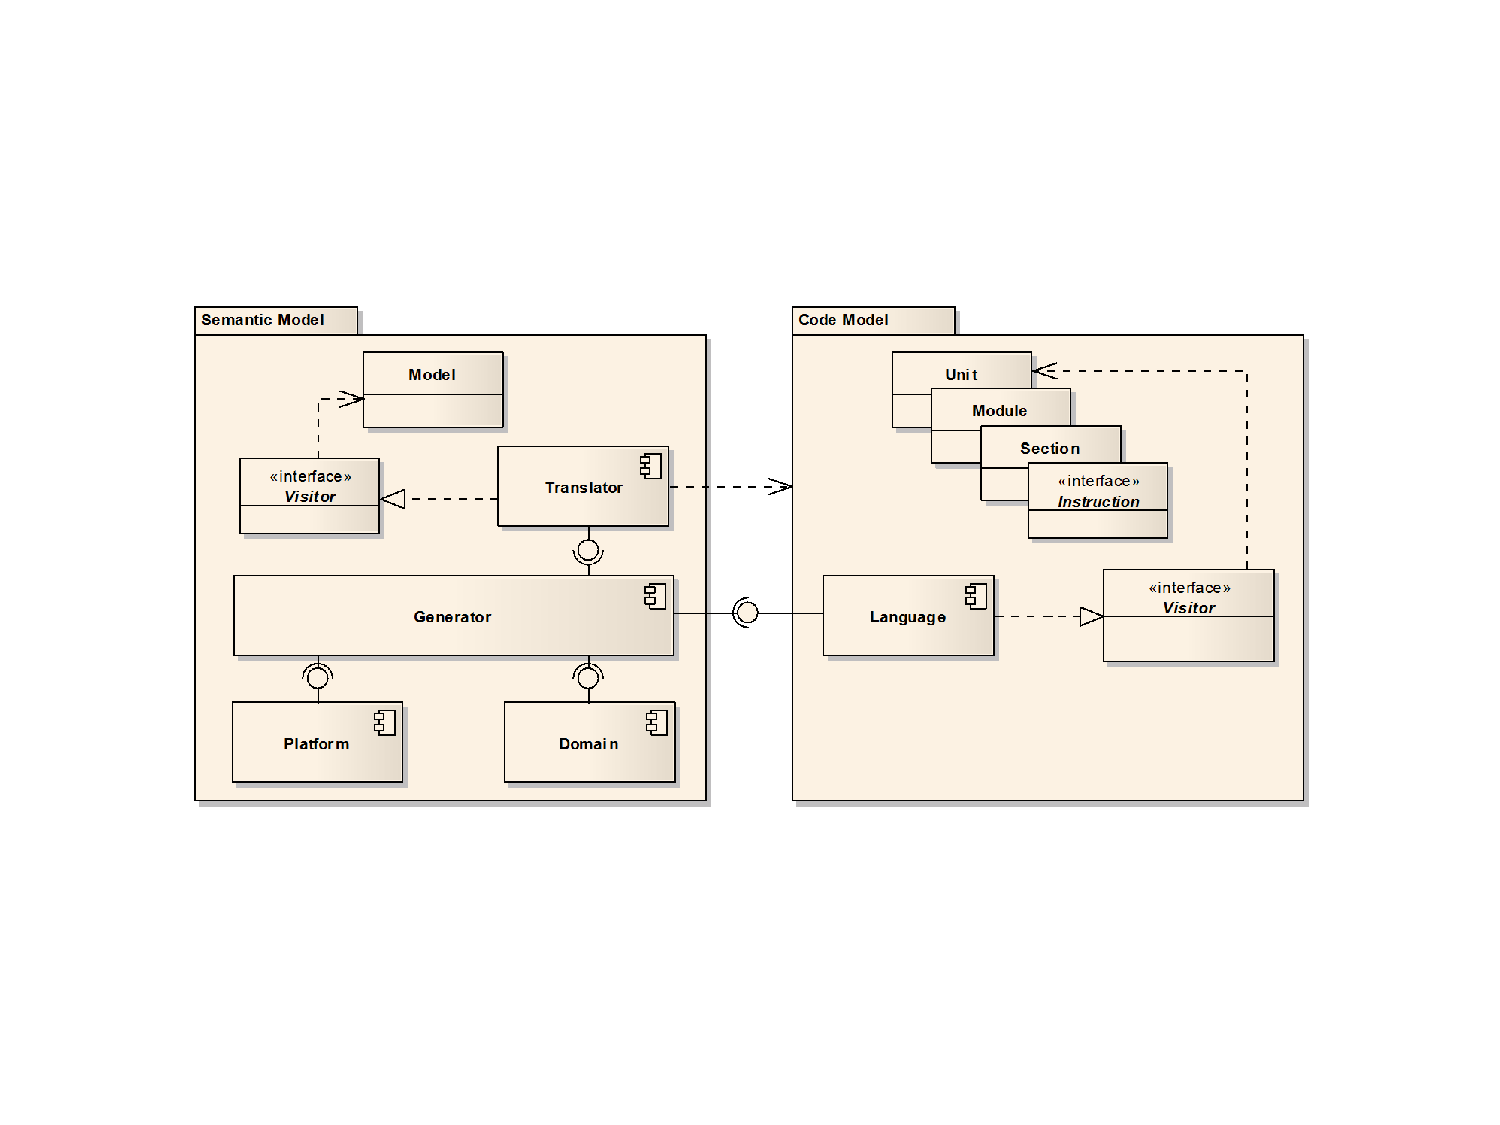
\includegraphics[width=\linewidth]{resources/component-overview.pdf}
  \caption{Overzicht van componenten en kernentiteiten}
  \label{fig:devel-component-overview}
\end{figure}

Intern bestaat de oplossing uit twee grote delen: het semantische en het
code-gedeelte. Binnen het semantische gedeelte vinden we het SM terug. Dit
model kan benaderd worden door middel van een zgn. \emph{visitor}, een
implementatie van het \emph{visitor}-patroon. Aan de hand van deze
\emph{visitor} kunnen transformaties van het model gerealiseerd worden.

Het SM is de primaire invoer voor de generator. Deze kan zijn taak slechts
vervullen door middel van een compositie met een \emph{platform-} en
\emph{domeinindefinitie}, een vertaler (\emph{Translator}) die elementen uit
het semantische gedeelte kan omzetten naar overeenkomstige elementen in het
code-gedeelte, en de uiteindelijk beoogde programmeertaal (\emph{Language}).

De programmeertaal maakt deel uit van het code-gedeelte, wat in hoofdzaakhet CM
bevat. Dit is op zijn beurt opgebouwd uit een hi\"erarchie van vier niveaus. De
structuur van de beoogde code wordt weergegeven door de compilatie \emph{unit},
de \emph{modules} en de \emph{secties}. Hier staat de unit voor het geheel, de
modules voor functioneel samenhangende delen en de secties voor een fysieke
opdeling in bestanden. De juiste realisatie van deze hi\"erarchie wordt
overgelaten aan de implementatie van de taal die hier betekenis aan kan geven.

Op het laagste niveau van het CM vinden we de \emph{instructies}. Deze kunnen
gebruikt worden om effectieve code voor te stellen. Er bestaat in het CM per
definitie een overeenkomstige instructie voor elk element uit het SM. Aangezien
het SM functioneel rijker is dan de meeste programmeertalen, moeten na
constructie van het initi\"ele CM, door middel van transformaties,
alternatieven ge\"implementeerd worden, die binnen de mogelijkheden van de
uiteindelijke programmeertaal liggen.

\subsection{ANTLR}
\label{subsection:devel-antlr}

Het generatieproces start met het inladen van de FOO-lang-bronbestanden in het
SM. Dit gebeurt door middel van een \emph{parser} die de tekstuele voorstelling
analyseert en de semantische constructies detecteert. Het resultaat van deze
stap is een boomstructuur die de betekenis van de verschillende constructies
structureel weergeeft. Zo'n boomstructuur is een AST. Figuur
\ref{fig:devel-ast} toont de AST van het elementaire voorbeeld uit
codevoorbeeld \ref{lst:hello.foo}.

\begin{figure}[ht]
  \centering
  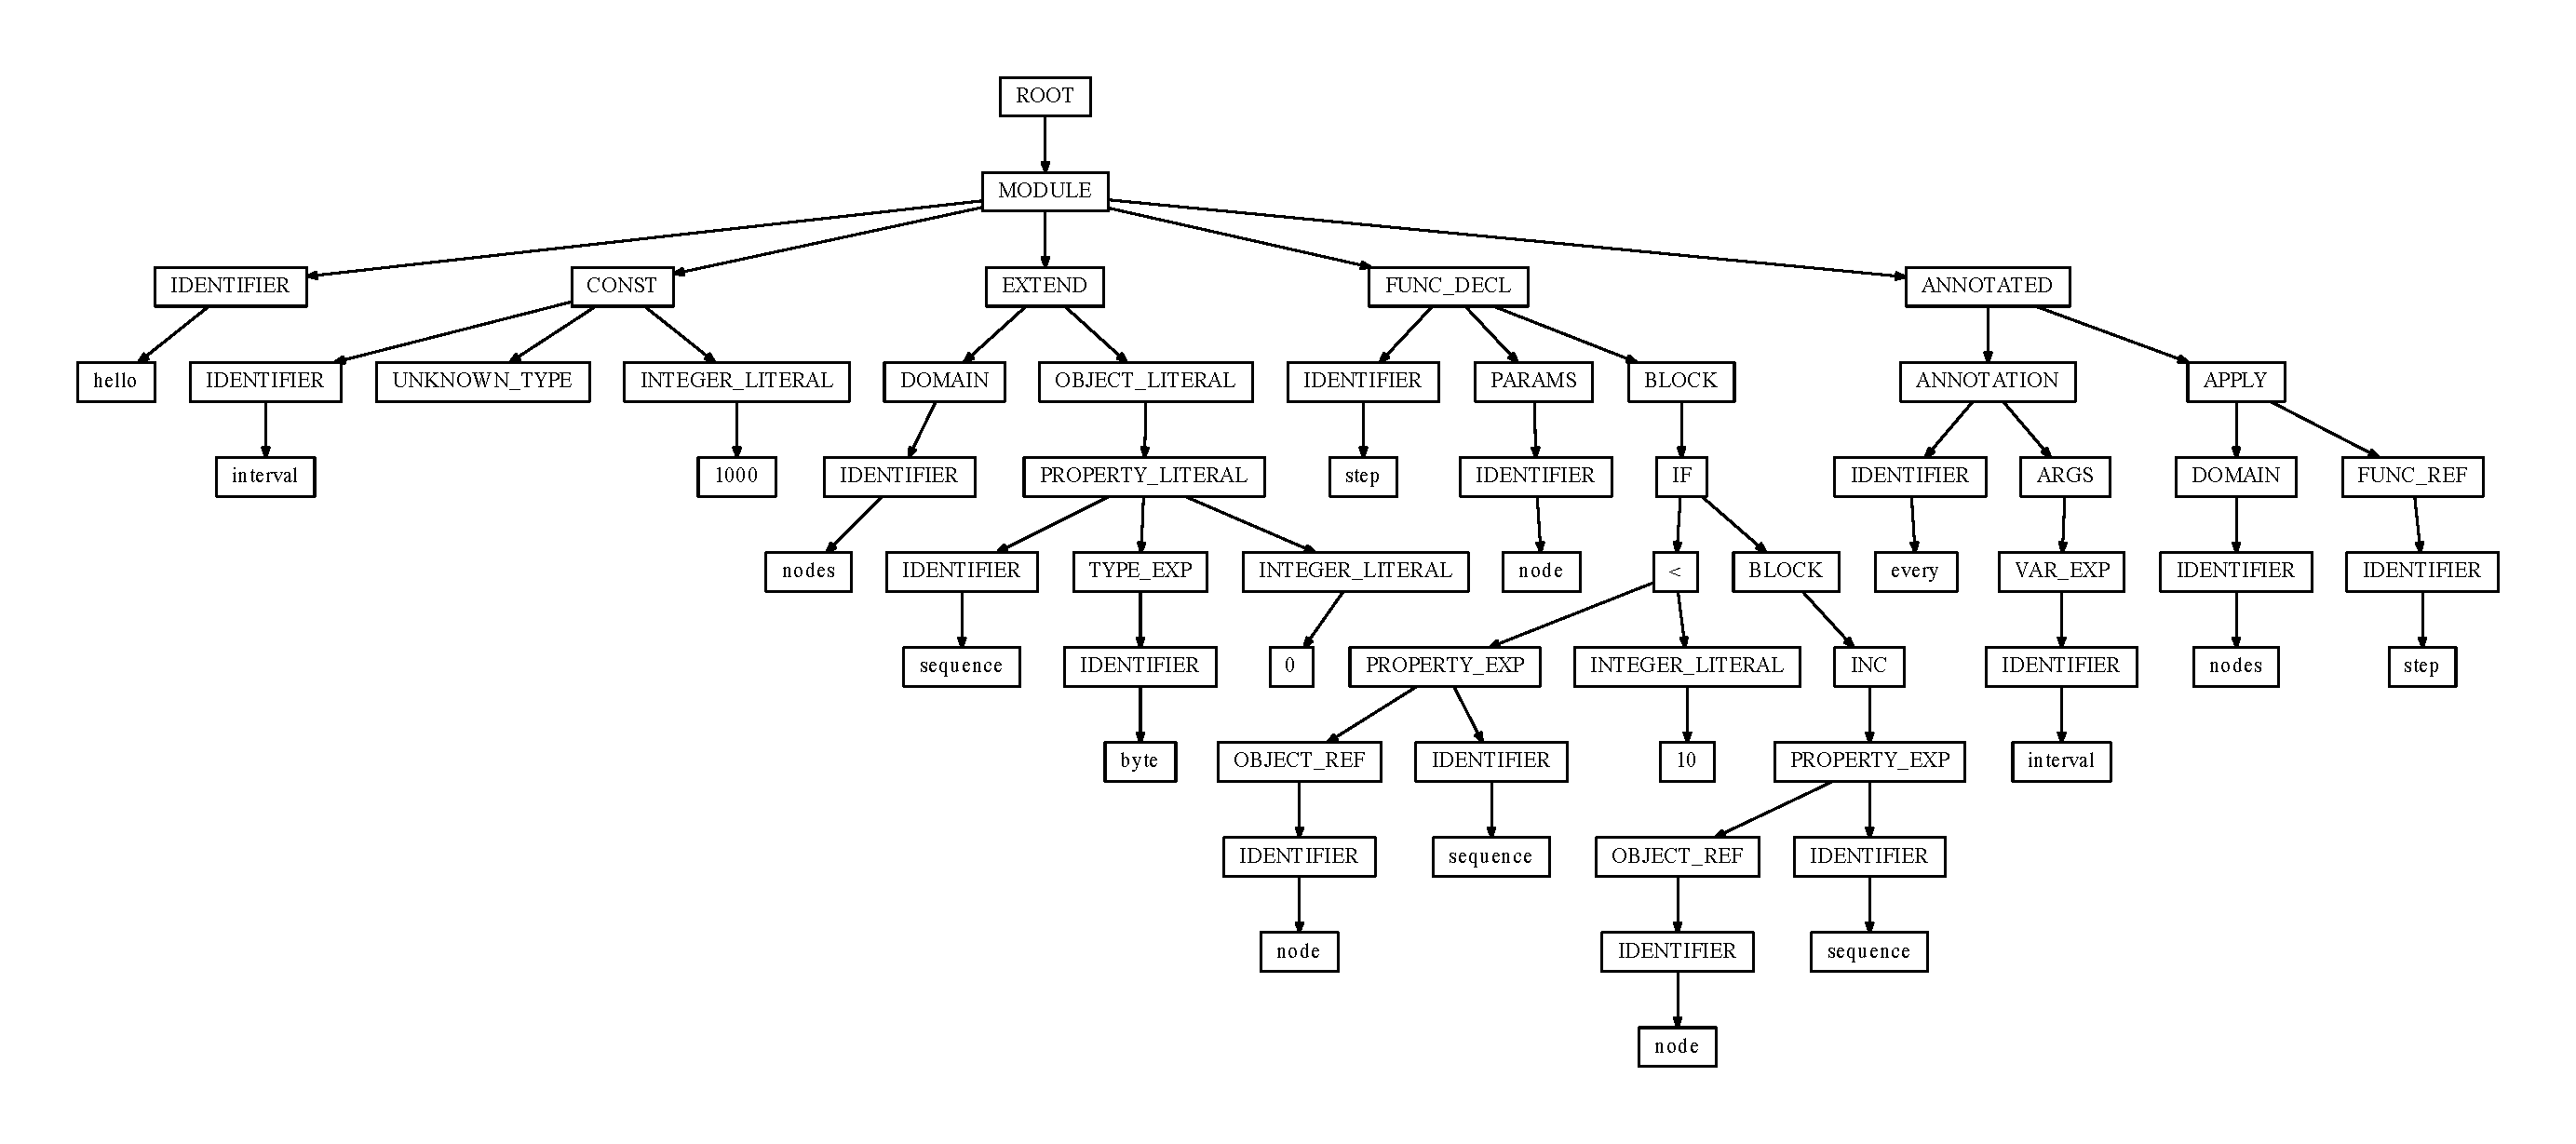
\includegraphics[width=\linewidth]{resources/hello_ast.pdf}
  \caption{De AST van het elementaire voorbeeld, \ttt{hello.foo}}
  \label{fig:devel-ast}
\end{figure}

We herkennen de inhoud van het codevoorbeeld in deze figuur: op het hoogste
niveau zien we de module met een naam (\ttt{IDENTIFIER}), de definitie van een
constante (\ttt{CONST}), een uitbreiding van het domein (\ttt{EXTEND}), een
functiedefinitie (\ttt{FUNC\_DECL}) en een geannoteerde applicatie
(\ttt{ANNOTATED}) van een functie op een domein. De AST is ontdaan van alle
ondersteunende syntax, zoals aanduidingen voor blokken code\dots en bevat
louter de semantische inhoud.

%!TEX root=masterproef.tex

\subsection{Interfaces}
\label{subsection:devel-codegen-interfaces}

Voor we het SM en het CM in detail bekijken, kijken we eerst naar de interfaces
die de codegenerator ter beschikking stelt.

\subsubsection{foo.py}

Op het hoogste niveau biedt de generator een interface via de opdrachtprompt
(\emph{Command-Line Interface}) (CLI) aan in de vorm van een Python script:
\ttt{foo.py}. Codevoorbeeld \ref{lst:foo.py-help} toont de uitvoering van het
script en geeft een overzicht van de mogelijkheden.

\begin{listing}[ht]
  \begin{minted}[linenos,frame=lines,framesep=2mm,fontsize=\footnotesize]{console}
$ source setpath.sh
$ ./foo.py --help
usage: foo.py [-h] [-v] [-c] [-i] [-g FORMAT] [-o OUTPUT] [-l LANGUAGE]
              [-p PLATFORM]
              [sources [sources ...]]

Command-line tool to interact with foo-lang and its code generation
facilities.

positional arguments:
  sources               the source files in foo-lang

optional arguments:
  -h, --help            show this help message and exit
  -v, --verbose         output info on what's happening
  -c, --check           perform model checking
  -i, --infer           perform model type inferring
  -g FORMAT, --generate FORMAT
                        output format (choices: none, ast, ast-dot, sm-dot,
                        foo, code / default: none)
  -o OUTPUT, --output OUTPUT
                        output directory (default: .)
  -l LANGUAGE, --language LANGUAGE
                        when format=code: target language (choices: c /
                        default: c)
  -p PLATFORM, --platform PLATFORM
                        when format=code: target platform (choices: moose,
                        demo / default: moose)
  \end{minted}
  \vspace{-5mm}
  \caption{Informatie over de werking van \ttt{foo.py}}
  \label{lst:foo.py-help}
\end{listing}

De CLI biedt toegang tot alle aspecten van de generator: modelcontrole
(\ttt{check}), typedeductie (\ttt{infer}), het uitvoerformaat (\ttt{format}),
plaats van de uitvoer (\ttt{output}), de programmeertaal (\ttt{language}) en
voor welk platform de generatie moet gebeuren (\ttt{platform}).

De lijst van mogelijke uitvoerformaten bestaat uit: \ttt{none}, \ttt{ast},
\ttt{ast-dot}, \ttt{sm-dot}, \ttt{foo} en \ttt{code}. Formaat \ttt{ast} toont
een hi\"erarchisch overzicht van de AST op het scherm in tekstuele vorm. De
uitvoer van \ttt{ast-dot} zagen we eerder in figuur \ref{fig:devel-ast}. De
uitvoer is code die als invoer kan dienen voor GraphViz \citep{url:graphviz},
een openbronproject dat zich specialiseert in het visualiseren van
graafgeori\"enteerde gegevens, zoals deze AST. Door middel van het
\ttt{dot}-commando kan van deze code een visuele voorstelling gemaakt worden.

Overeenkomstig bestaat er de mogelijkheid om een visuele voorstelling te maken
van het SM, door middel van het \ttt{sm-dot} formaat. Om controles te doen
betreffende de goede verwerking van de FOO-lang broncode kan een ingelezen set
van modules ook opnieuw als FOO-code uitgevoerd worden.

Tot slot is er nog het \ttt{code} formaat, dat de generator vraagt om code te
genereren. Hierbij dienen dan ook de overige opties voorzien te worden:
uitvoerlocatie, taal en platform.

\subsubsection{API}

Het \ttt{foo.py} Python-script is slechts een dunne schil rond de Python-API.
Deze biedt alle functionaliteit aan in de vorm van een Python-module met een
imperatieve interface. Codevoorbeeld \ref{lst:codegen-api} toont de interface
van deze module.

\begin{listing}[ht]
  \begin{minted}[linenos,frame=lines,framesep=2mm,fontsize=\footnotesize]{python}
def create_model():
  ...
  return model

def parse(string, noprint=False):
  ...
  return parser

def infer(model, silent=False):
  ...

def check(model, silent=False):
  ...

def generate(model, args):
  ...

def load(string, model=None):
  ...
  return model
  \end{minted}
  \vspace{-5mm}
  \caption{API van de codegenerator}
  \label{lst:codegen-api}
\end{listing}

De verschillende fasen uit het generatieproces bestaan uit het aanmaken van een
(leeg) model, het parsen van de broncode, het deduceren van onbekende types,
het controleren of een model volledig in orde is en het genereren van code. De
bijkomende \ttt{load}-functie combineert de \ttt{create\_model} en
\ttt{parse}-functionaliteit in \'e\'en handige functie.

De API laat toe om de generator vanuit Python aan te spreken en eventueel
verder te integreren in een uitgebreider compilatieproces, of om andere
interfaces te voorzien (visuele gebruikersinterfaces zoals bv. een
webinterface\dots).

Verder biedt de API toegang tot de entiteiten op het hoogste niveau, zoals de
parser, de model-entiteit uit het SM\dots De volledige openheid van Python-code
laat toe om dieper door te dringen en elk aspect van het model te ondervragen
en te wijzigen.

Beide onderliggende modellen kunnen tevens volledig benaderd worden aan de hand
van een \emph{visitor}. Deze wordt door de generator veelvuldig gebruikt, zelfs
voor kleine operaties en biedt een aantrekkelijkere interface om met de
modellen te werken dan het direct ondervragen van eigenschappen en het
aanroepen van methoden in het model.

%!TEX root=masterproef.tex

\subsection{Semantisch model}
\label{subsection:devel-semantic-model}

De AST wordt door een eerste \emph{visitor} ingeladen in het SM. Dit is in
essentie een eenvoudige vertaling van de boomstructuur naar de overeenkomstige
elementen in het SM. Het resultaat kan gevisualiseerd worden door middel van
GraphViz, zoals weergegeven in figuur \ref{fig:hello.sm}.

\begin{figure}[ht]
  \centering
  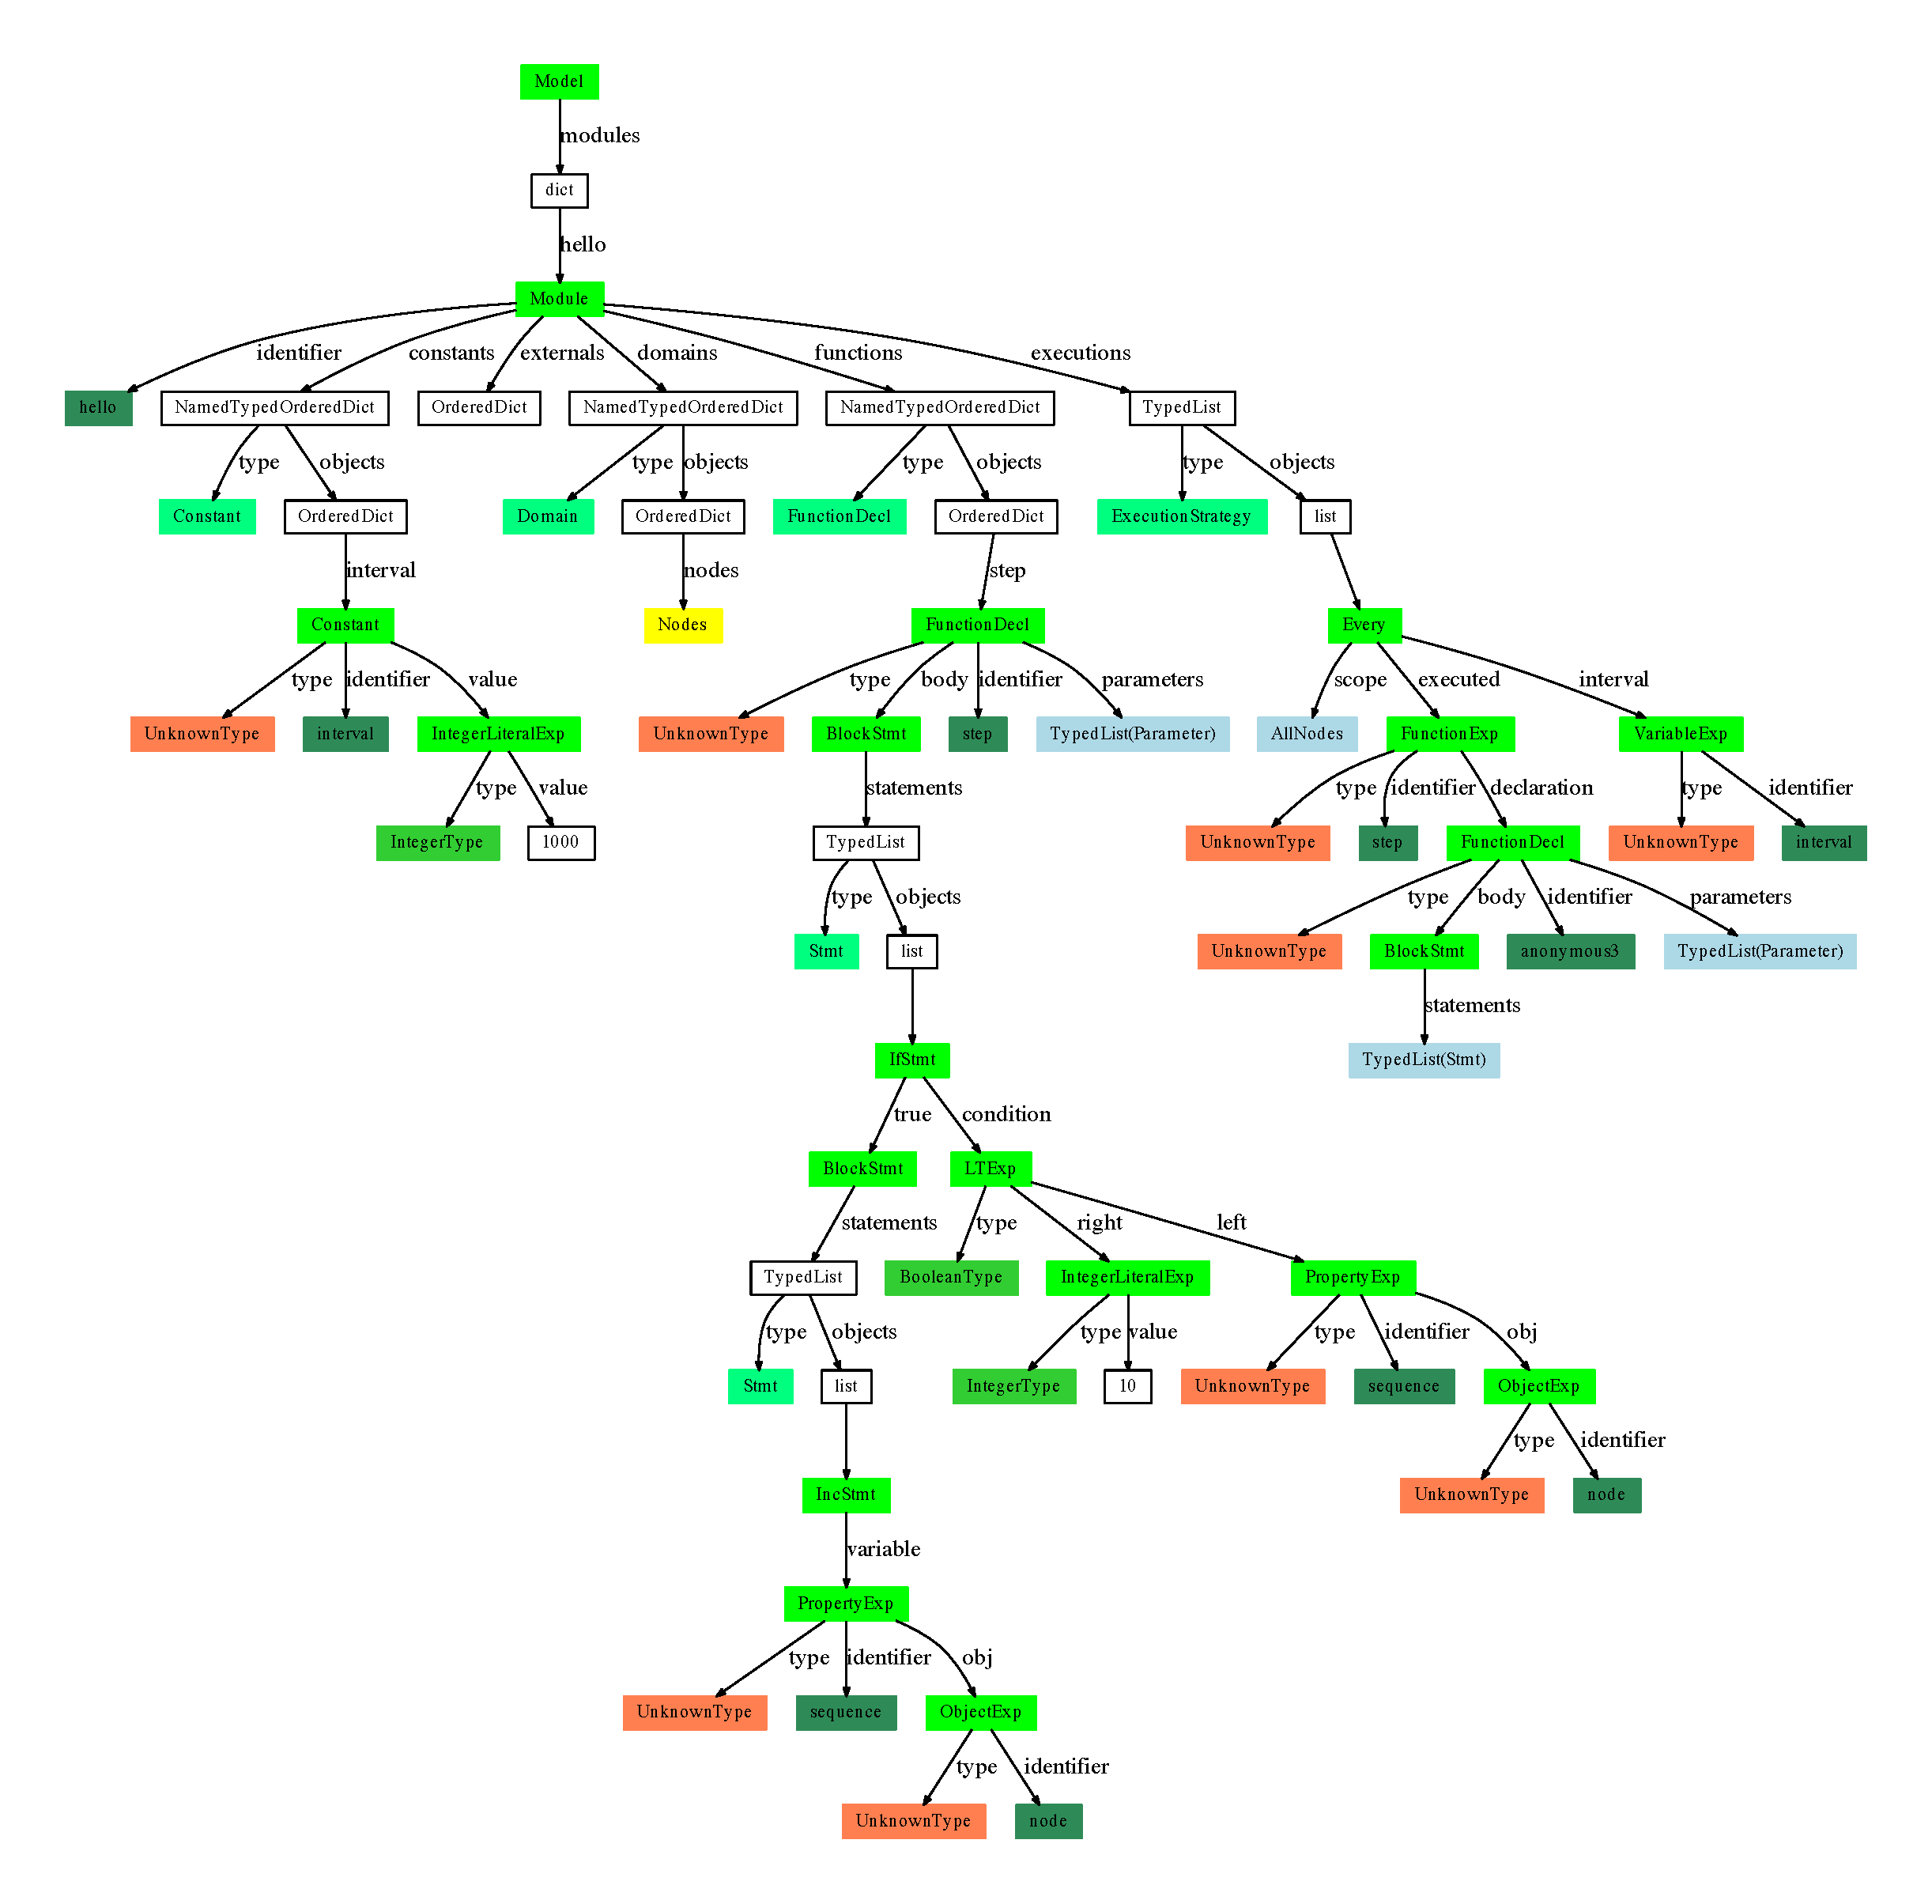
\includegraphics[width=\linewidth]{resources/hello_sm.pdf}
  \caption{Het SM van het elementaire voorbeeld, \ttt{hello.foo}}
  \label{fig:hello.sm}
\end{figure}

Het SM bevat meer informatie dan de AST, zoals bv. typering. Bij deze
visualisatie is gebruikgemaakt van een kleurencodering. Hierdoor wordt het
makkelijker om het diagram te interpreteren.

De belangrijkste kleur is zonder meer de rode kleur, die problemen in het model
aangeeft. In dit geval betreft het onbekende types. Dit is in deze fase van het
generatieproces normaal aangezien typering in FOO-lang optioneel is. Deze
eerste versie van het SM bevat daarom nog niet alle types.

Een ander deel dat lijkt te ontbreken in dit diagram is de uitbreiding van het
domein. In het voorbeeld werd immers een eigenschap \ttt{sequence} toegevoegd.
Aangezien dit een uitbreiding is van het domein, zal deze terug te vinden zijn
in de eigen instantie van het domein voor deze module. In figuur
\ref{fig:hello.sm} is dit domein beperkt tot een referentie in een gele kleur.
De volledig inhoud van wat hierachter schuil gaat, is opgenomen in bijlage
\ref{section:nodes.sm}.

Dit is een groot stuk van het SM en behelst verschillende types en
functiedeclaraties die door het \ttt{nodes}-domein ge\"introduceerd worden in
het SM. Hier vinden we tevens de uitbreiding met de extra \ttt{sequence}
eigenschap.

\vspace{-3mm}

\subsubsection{Type deductie}

De volgende stap in het generatieproces bestaat erin om de nog onbekende types
te deduceren op basis van andere informatie uit het SM. Dit gebeurt aan de hand
van de \ttt{inferrer}-module. Dit is een implementatie van de \emph{visitor}
voor het SM die nagaat of alle types gekend zijn. Voor onbekende types wordt,
afhankelijk van de plaats van het type op verschillende manieren op zoek gegaan
naar een juiste typering.

De eenvoudigste methode bouwt, terwijl het model doorlopen wordt, een overzicht
op van gekende types die ontstaan door de declaratie van variabelen\dots Indien
een onbekend type wordt gevonden, consulteert de \ttt{inferrer}-module dit
overzicht. Indien een referentie naar een eerdere declaratie gevonden wordt,
kan het type eenvoudig gededuceerd worden.

In een aantal gevallen is de deductie niet rechtstreeks af te lezen uit
declaraties en moet er naar andere mogelijke combinaties gekeken worden.
Voorbeelden hiervan zijn bv. functiedeclaraties die gebruikt worden als reactie
op een gebeurtenis. De gebeurtenis specificeert hoe de reagerende functie
gedeclareerd is. Op basis van de omkaderende gebeurtenis moet vervolgens het
overeenkomstige prototype van de functie opgezocht en gekoppeld worden.

Na het succesvol uitvoeren van deze type-deductie zijn alle voorheen onbekende
types gekend en is het model volledig. Figuur \ref{fig:hello.sm-inferred} toont
hetzelfde SM als voordien, echter nu met volledig gekende typering.

\begin{figure}[ht]
  \centering
  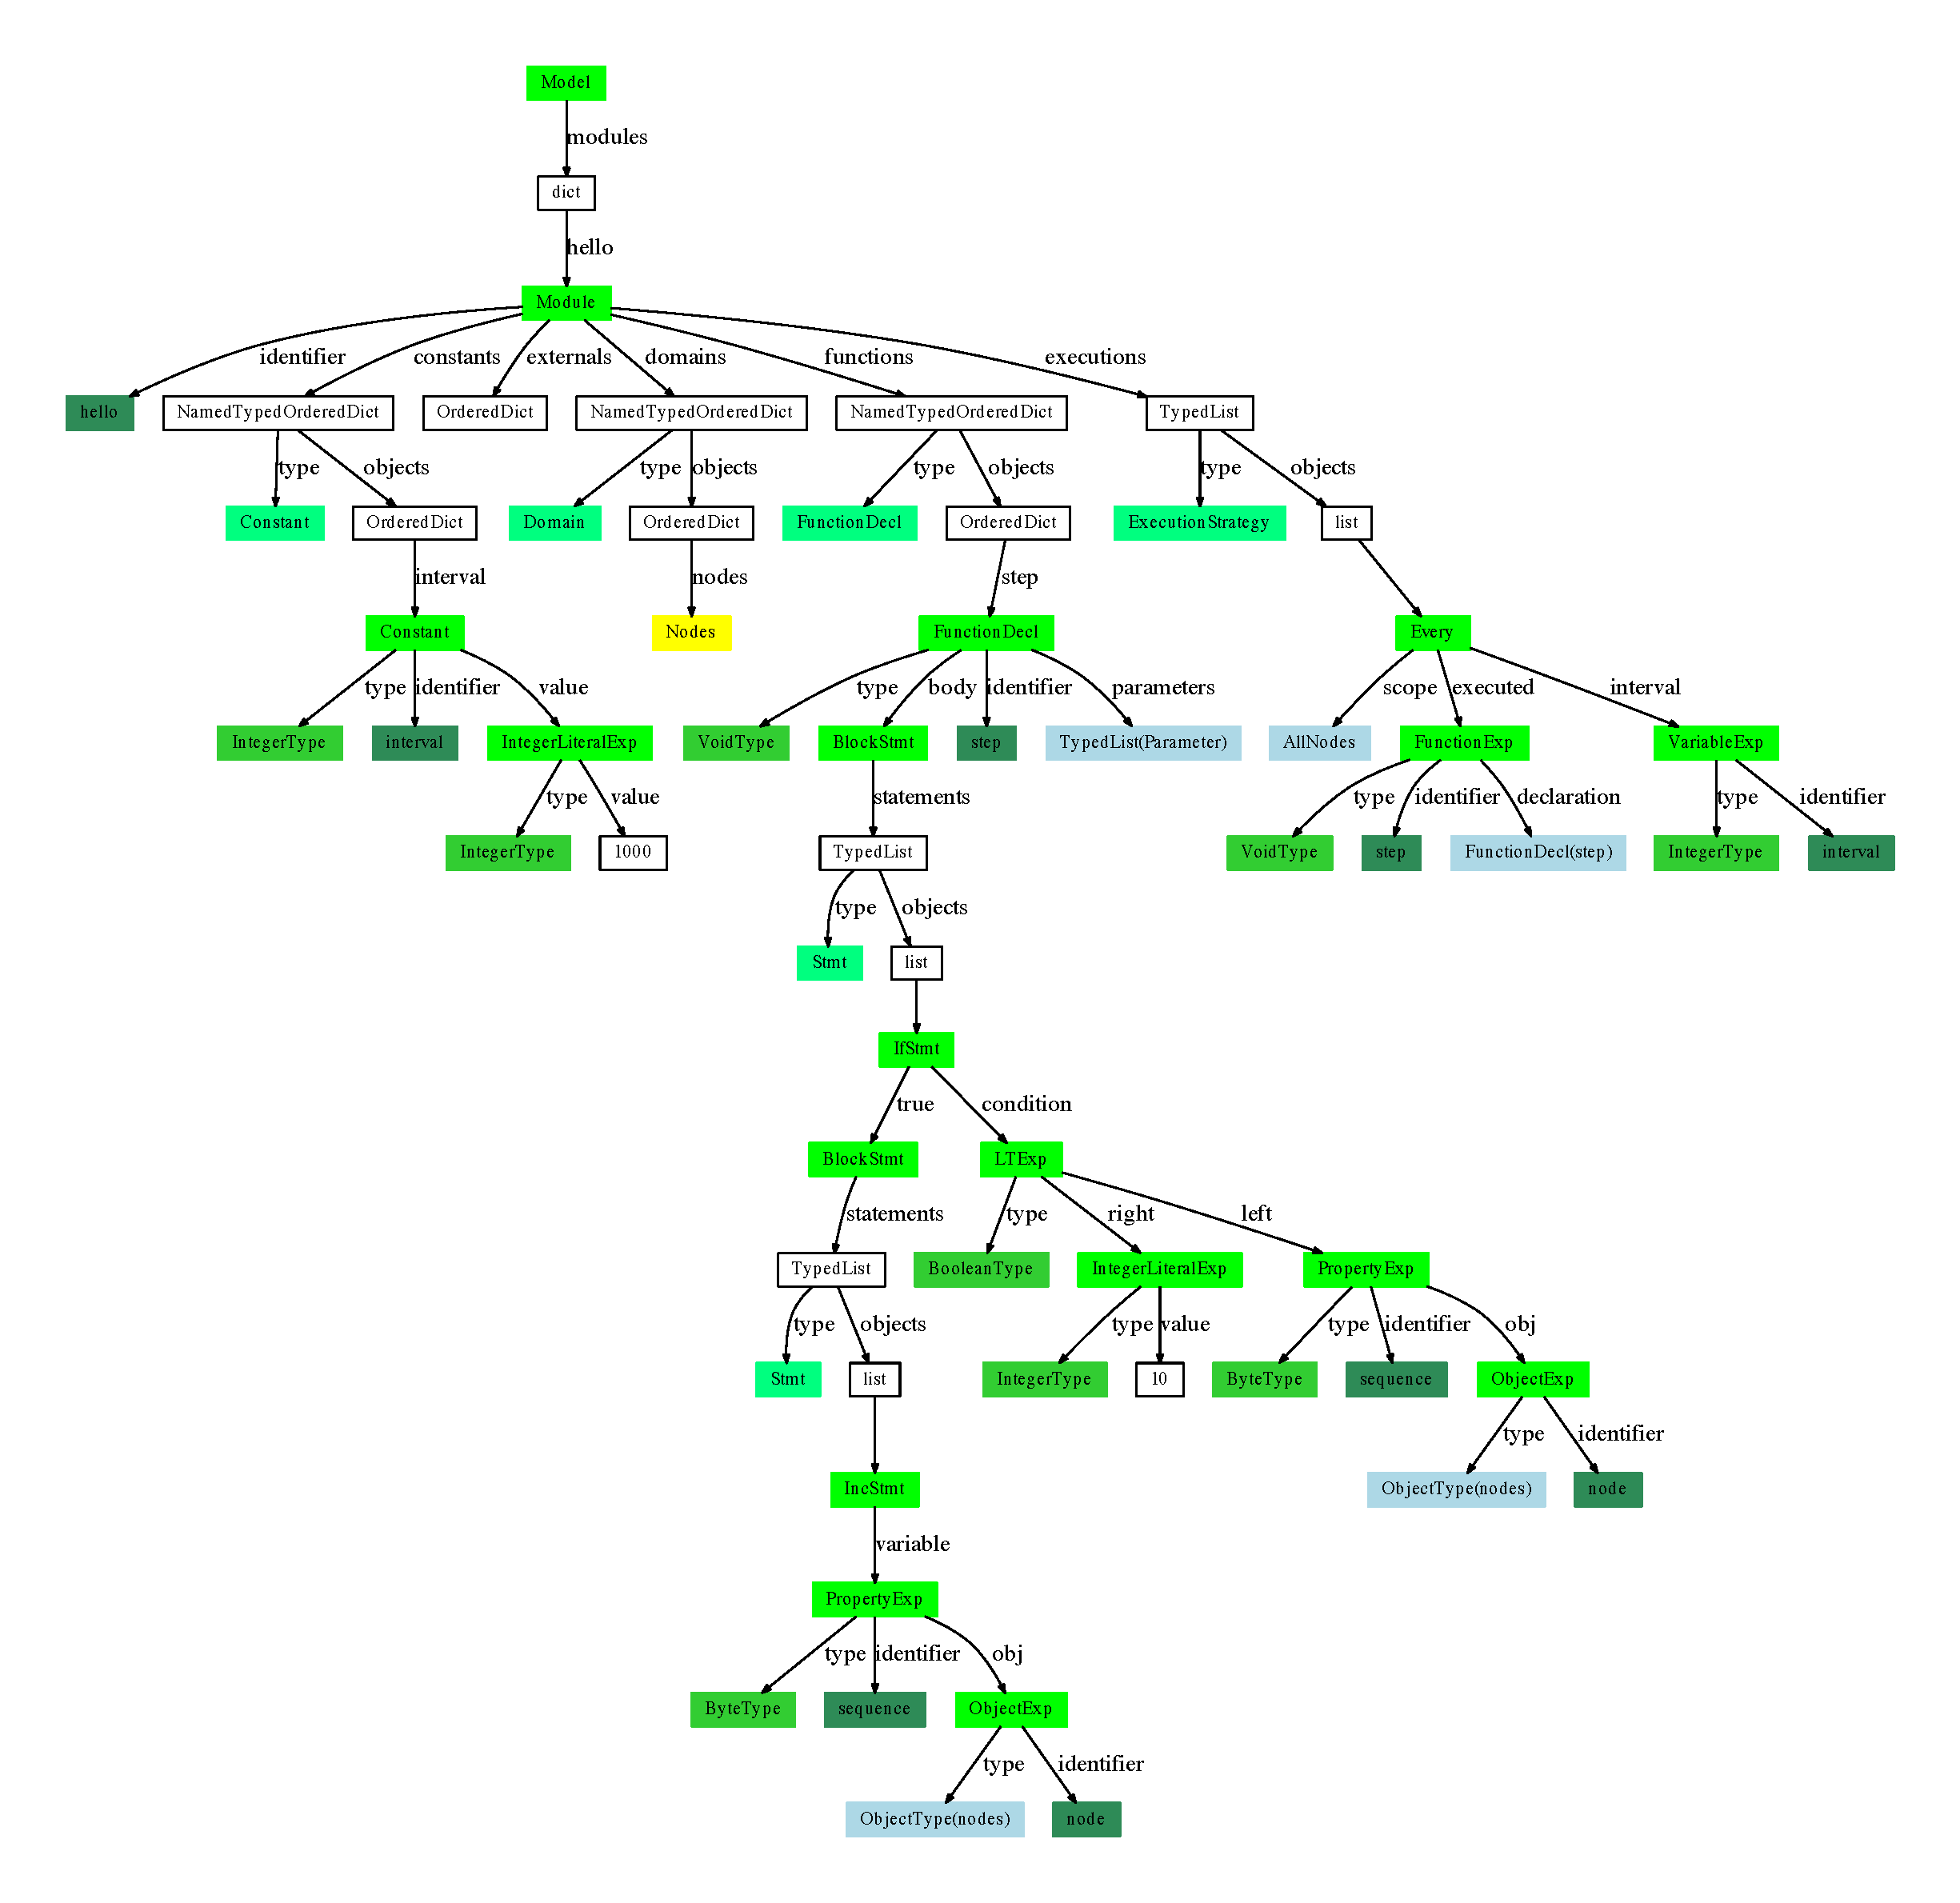
\includegraphics[width=\linewidth]{resources/hello_sm_inferred.pdf}
  \caption{Het SM van het elementaire voorbeeld, \ttt{hello.foo}, na type deductie}
  \label{fig:hello.sm-inferred}
\end{figure}

Ofschoon men verwacht dat deze fase geen structurele wijzigingen aanbrengt aan
het SM, zien we in dit geval toch dat er een vijftal elementen uit het model
verdwenen lijken te zijn. Dit is nochtans een gewoon voorbeeld van deductie. Na
het inladen van het initi\"ele model werd de (enige) uitvoeringsstrategie
gekoppeld aan een functie-expressie (\emph{FunctionExp}) genaamd \ttt{step}. Op
dat ogenblik was er over \ttt{step} niets meer geweten. De declaratie van
\ttt{step} was wel eerder gebeurd, maar het is pas in de deductiefase dat het
onbekende type van deze functie opgezocht werd. Deel van het type is tevens de
declaratie ervan. Tijdens de deductiefase wordt deze gekoppeld aan de eerdere
declaratie, waardoor in figuur \ref{fig:hello.sm-inferred} deze
functiedeclaratie niet meer volledig getoond wordt, maar nu als een referentie
naar de \ttt{step} functie opgenomen is.

\vspace{-3mm}

\subsubsection{Model controle}

De \ttt{inferrer}-module tracht alle onbekende types te deduceren. Een tweede
ondersteunende module is de \ttt{checker}-module of modelcontrole. Deze
overloopt aan de hand van een \emph{visitor} het hele model en controleert of
alles in orde is.

De \ttt{checker}-module is typisch nuttig bij het schrijven van FOO-lang code
en kan dienen als syntactische en semantische controle. Wanneer er bv. een
schrijffout gemaakt wordt in de naam van een variabele of functie, kan dit soms
niet direct opvallen. FOO-lang maakt bv. automatisch declaraties voor
variabelen aan wanneer zij voor het eerst gebruikt worden en nog niet eerder
gedeclareerd werden. De \ttt{checker}-module kan bv. voor deze situaties
waarschuwingen geven, die kunnen helpen bij het schrijven van de FOO-lang
broncode.

%!TEX root=masterproef.tex

\subsection{Code model}
\label{subsection:devel-code-model}

Het CM staat in feite volledig los van de generator en het SM en is ook als een
op zich staand project ontwikkeld als generieke beschrijving van uitvoerbare
code, genaamd \emph{CodeCanvas}.

\subsubsection{CodeCanvas}

CodeCanvas biedt een API om hi\"erarchische structuren te bouwen. Deze kunnen
opgebouwd worden uit zelf te defini\"eren entiteiten bestaan. Standaard
voorziet CodeCanvas de concepten \emph{unit}, \emph{module} en \emph{sectie}.

Een \emph{unit} is het hoogste niveau en verzamelt alle onderliggende
\emph{modules}. Een \emph{module} komt overeen met een functioneel geheel en
bestaat standaard uit twee \emph{secties}, \'e\'en voor declaraties en \'e\'en
voor definities. Een \emph{sectie} kan verder ingevuld worden met \emph{code
instructies}.

Daarnaast biedt CodeCanvas de mogelijkheid om entiteiten te markeren met een
label (\emph{tag}) en onderliggende entiteiten te selecteren of zoeken
op basis van die labels.

Dankzij een \emph{vloeiende} (\emph{fluent}) interface laat CodeCanvas
toe om zeer leesbare operaties te formuleren op deze hi\"erarchische
codestructuren.

Codevoorbeeld \ref{lst:codecanvas-hello} toont een eenvoudig voorbeeld dat de
meeste functionaliteit toepast. 

\begin{listing}[ht]
  \begin{minted}[linenos,frame=lines,framesep=2mm,fontsize=\footnotesize]{python}
from structure import Unit, Module
import instructions as code
import languages.C  as C

unit = Unit().append( Module("hello") )
main = unit.select("hello", "dec").append(code.Function(name="main"))
main.append(code.Print("Hello World\n"))

print str(unit)
print C.Emitter().emit(unit)
print str(unit)
  \end{minted}
  \vspace{-5mm}
  \caption{Werking van het \emph{CodeCanvas}}
  \label{lst:codecanvas-hello}
\end{listing}

Het voorbeeld construeert op regel 5 een \emph{unit} aan en voegt er een
\emph{module} genaamd \ttt{hello} aan toe. Achterliggend worden bij de aanmaak
van een module onmiddellijk 2 \emph{secties} toegevoegd, genaamd \ttt{dec} en
\ttt{def}.

Op regel 6 wordt vertrekkende van de \emph{unit} de \ttt{dec} \emph{sectie}
geselecteerd. De \ttt{select} methode laat toe om een opeenvolgende reeks van
\emph{labels} te defini\"eren die het pad vormen vanaf de startentiteit tot de
te selecteren entiteit.

Een gelijkaardige methode, \ttt{find}, accepteert ook een variabele lijst
argumenten en zoekt vervolgens, vertrekkende van de startentiteit, naar
entiteiten die alle opgegeven \emph{labels} dragen.

Beide methodes kunnen lijsten van entiteiten teruggeven. Op deze lijsten kunnen
evengoed alle methoden opgeroepen worden als op een enkele entiteit. Dit
resulteert in een zeer transparante interface.

De geselecteerde sectie wordt vervolgens een functie toegevoegd met de naam
\ttt{main}. Op regel 7 wordt aan deze functie een \ttt{print} opdracht
toegevoegd. Tot slot wordt de \emph{unit} op twee manieren uitgevoerd: eerst
door er een tekstuele voorstelling van te maken en in tweede instantie door
gebruik te maken van een programmeertaal, in dit geval C.

De uitvoer van dit programma is weergegeven in \ref{lst:codecanvas-output} en
toont eerst de technische tekstuele voorstelling van de hi\"erarchie. Tussen
vierkante haakjes staan de \emph{labels} die aan een entiteit verbonden zijn.
Effectieve instructie-implementaties tonen hun parameters als een verzameling
van de naam en de waarde.

\begin{listing}[ht]
  \begin{minted}[linenos,frame=lines,framesep=2mm,fontsize=\footnotesize]{console}
  Module hello [hello]
    Section def [def]
    Section dec [dec]
      Function {'params': (), 'type': void, 'id': main}
        Print {'args': (), 'string': "Hello World\n"}

  void main(void);
  #import <stdio.h>
  void main(void) {
    printf("Hello World\n");
  }
  
  Module hello [hello]
    Section def [def]
      Prototype {'params': [], 'type': void, 'id': main}
    Section dec [dec]
      Import {'imported': '<stdio.h>'} [import_stdio] <sticky>
      Function {'params': [], 'type': void, 'id': main}
        Print {'args': (), 'string': "Hello World\n"}
  \end{minted}
  \vspace{-5mm}
  \caption{Uitvoer van voorbeeld werking van het \emph{CodeCanvas}}
  \label{lst:codecanvas-output}
\end{listing}

Het tweede deel van de uitvoer toont de overeenkomstige C code voor deze
hi\"erarchie. We merken hier op dat op regel 7 een prototype en op regel 8 een
\emph{import} opdracht verschijnen die niet in de hi\"erarchie voorkwamen.

Wanneer we een tweede maal de \emph{unit} omvormen tot een tekstuele
voorstelling, zien we deze twee entiteiten wel opduiken. De uitvoermodule voor
de C programmeertaal werkt in meerdere stappen. 

Tijdens een eerste fase wordt de hi\"erarchie doorlopen en worden uitbreidingen
gedaan. In dit voorbeeld gebeuren er twee: wanneer een \emph{print} opdracht
gevonden wordt, wordt een \emph{import} opdracht toegevoegd die de declaraties
van \ttt{stdio.h} zal inladen. Een tweede transformatie zal voor elke
\emph{functie} een prototype aanmaken in de declaratie sectie van de module.

Deze fase zorgt ook voor het omzetten van constructies die niet standaard
ondersteund worden naar uitwerkingen met constructies die wel bestaan bij de
beoogde taal. Een voorbeeld hiervan zijn bv. \emph{tuples}. Deze worden door de
omvormer van C herschreven door middel van structuren en functies om deze
structuren te benaderen en onderhouden.

In een tweede fase doorloopt de uitvoermodule opnieuw de volledige
hi\"erarchie, maar vormt nu elke entiteit om in de overeenkomstige tekstuele C
syntax.

Beide fasen worden ge\"implementeerd door middel van \emph{visitors}. Deze
\emph{visitor} is tevens beschikbaar van buitenaf en laat toe om andere
transformaties te implementeren.

\subsubsection{Filosofie}

De doelstelling van CodeCanvas is het aanbieden van een API die toelaat om te
werken zoals zoals programmeur denkt/werkt tijdens programmeren, maar nu op
basis van een abstracte programmeertaal die een superset aanbiedt van
constructies uit verschillende programmeertalen.

Enkele typische eigenschappen die deze doelstelling ondersteunen zijn:

\begin{description}

  \item[Functionele cross-referenties] - Door middel van \emph{labels} en de
  \emph{selectie} en \emph{zoek} functionaliteit kan er op functionele wijze
  omgegaan worden met code. Zo kan een gebruiker een in de beschrijving van een
  functie een \emph{label} toevoegen en hier later eenvoudig naar verwijzen om
  nog bijkomende logica toe te voegen.

  \item[Zoek-en-wijzig] - Dankzij de functionele cross-referenties en de
  transparantie van een enkele entiteit of een lijst van entiteiten is het heel
  eenvoudig om algemene aanpassingen door te voeren. Dit kan bv. gebruikt
  worden om aan het begin van alle declaratie-secties een standaard blok
  commentaar te plaatsen of om systematisch aanpassingen met betrekking tot
  naamgeving door te voeren.

  \item[Automatische vervolledigen] - Het voorbeeld van het automatisch
  toevoegen van \ttt{import} opdrachten of \ttt{prototypes} bieden een
  krachtige manier om de gebruiker te ontslaan van redundant en repetitief werk.

\end{description}

%!TEX root=masterproef.tex

\subsection{Transformaties}
\label{subsection:transformations}

\TODO

\subsubsection{Het visitor patroon}
\label{subsubsection:devel-visitor-pattern}

\TODO

